\documentclass[13pt]{beamer}
%
% Choose how your presentation looks.
%
% For more themes, color themes and font themes, see:
% http://deic.uab.es/~iblanes/beamer_gallery/index_by_theme.html
%
\mode<presentation>
{
\usetheme{CambridgeUS}     % or try Darmstadt, Madrid, Warsaw, ...
\usecolortheme{beaver} % or try albatross, beaver, crane, ...
\usefonttheme{default}  % or try serif, structurebold, ...
\setbeamertemplate{navigation symbols}{}
\setbeamertemplate{caption}[numbered]
} 

\usepackage[english]{babel}
\usepackage[utf8x]{inputenc}
\usepackage{xcolor}
\usepackage{multicol}
\usepackage{tikz}
\usepackage{tikz-uml}
\tikzumlset{font=\footnotesize\ttfamily}
\usepackage{hyperref}

\usepackage{listings}
\definecolor{codegreen}{rgb}{0,0.6,0}
\definecolor{codegray}{rgb}{0.5,0.5,0.5}
\definecolor{codepurple}{rgb}{0.58,0,0.82}
\definecolor{backcolour}{rgb}{0.95,0.95,0.92}

\lstdefinestyle{myCustomCppStyle}{
language=C++,
numbers=left,
stepnumber=1,
numbersep=9pt,
tabsize=2,
showspaces=false,
showstringspaces=false
}

\lstset{basicstyle=\tiny,style=myCustomCppStyle}

\lstdefinestyle{mystyle}{
backgroundcolor=\color{backcolour},   
commentstyle=\color{codegreen},
keywordstyle=\color{magenta},
numberstyle=\tiny\color{codegray},
stringstyle=\color{codepurple},
basicstyle=\ttfamily\footnotesize,
breakatwhitespace=false,         
breaklines=true,                 
captionpos=b,                    
keepspaces=true,                 
numbers=left,                    
numbersep=5pt,                  
showspaces=false,                
showstringspaces=false,
showtabs=false,                  
tabsize=1
}

\lstset{style=mystyle}

\usepackage{graphicx}
\graphicspath{ {./images/} }

\usepackage{tikz}
\usetikzlibrary{decorations.text}
\usetikzlibrary{shapes.geometric, arrows, positioning, calc, matrix}

\tikzset{
basic box/.style={
shape=rectangle, rounded corners, align=center,
draw=#1, fill=#1!25},
header node/.style={
Minimum Width=header nodes,
font=\strut\Large\ttfamily,
text depth=+0pt,
fill=white, draw},
header/.style={%
inner ysep=+1.5em,
append after command={
\pgfextra{\let\TikZlastnode\tikzlastnode}
node [header node] (header-\TikZlastnode) at (\TikZlastnode.north) {#1}
node [span=(\TikZlastnode)(header-\TikZlastnode)] at (fit bounding box) (h-\TikZlastnode) {}
}
},
hv/.style={to path={-|(\tikztotarget)\tikztonodes}},
vh/.style={to path={|-(\tikztotarget)\tikztonodes}},
fat blue line/.style={ultra thick, blue}
}

\definecolor{mygray}{RGB}{208,208,208}
\definecolor{mymagenta}{RGB}{226,0,116}
\newcommand*{\mytextstyle}{\sffamily\Large\bfseries\color{black!85}}
\newcommand{\arcarrow}[3]{%
% inner radius, middle radius, outer radius, start angle,
% end angle, tip protusion angle, options, text
\pgfmathsetmacro{\rin}{1.7}
\pgfmathsetmacro{\rmid}{2.2}
\pgfmathsetmacro{\rout}{2.7}
\pgfmathsetmacro{\astart}{#1}
\pgfmathsetmacro{\aend}{#2}
\pgfmathsetmacro{\atip}{5}
\fill[mygray, very thick] (\astart+\atip:\rin)
                 arc (\astart+\atip:\aend:\rin)
-- (\aend-\atip:\rmid)
-- (\aend:\rout)   arc (\aend:\astart+\atip:\rout)
-- (\astart:\rmid) -- cycle;
\path[
decoration = {
 text along path,
 text = {|\mytextstyle|#3},
 text align = {align = center},
 raise = -1.0ex
},
decorate
](\astart+\atip:\rmid) arc (\astart+\atip:\aend+\atip:\rmid);
}
\title[Design Pattern]{Structural Design Pattern}
\author{Hung Tran}
\institute{Fpt software}
\date{\today}


\begin{document}

\begin{frame}
\titlepage
\end{frame}

% Uncomment these lines for an automatically generated outline.
\begin{frame}{Outline}
\tableofcontents
\end{frame}

\section{Structural Pattern Overview}

\begin{frame}{Structural Pattern Overview}
	\begin{center}
	\textcolor{blue}{\textbf{How classes and objects are composed fo form larger structure.}}
	\end{center}
	\begin{itemize}
		\item \textbf{Adapter}: Convert the interface of a class into another interface.
		\item \textbf{Bridge}: Decouple an abstraction from its implementation.
		\item \textbf{Composite}: Compose objects into tree structure.
		\item \textbf{Decorator}: Attach additional responsibilities to an object dynamically.
		\item \textbf{Facade}: Provide a unified interface to a set of interfaces.
		\item \textbf{Flyweight}: Use sharing to support large numbers of fine-grained objects efficiently.
		\item \textbf{Proxy}: Provide a surrogate or placeholder for another object to control access to it.
	\end{itemize}
\end{frame}

\section{Adapter pattern}

\begin{frame}{Problem Statement}
	\begin{columns}[T]
		\begin{column}{.5\textwidth}
			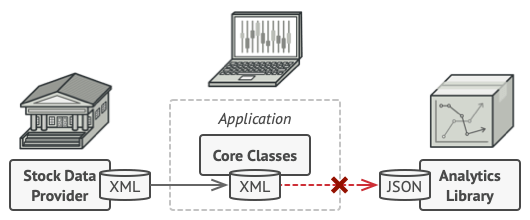
\includegraphics[scale=0.3]{./images/problem.png}
		\end{column}
	
		\begin{column}{.5\textwidth}
			\begin{itemize}
				\item Imagine that you’re creating a stock market monitoring app. The app downloads the stock data from multiple sources in XML format and then displays nice-looking charts and diagrams for the user.
				\item At some point, you decide to improve the app by integrating a smart 3rd-party analytics library. But there’s a catch: the analytics library only works with data in JSON format.
				\item You could change the library to work with XML. However, this might break some existing code that relies on the library. And worse, you might not have access to the library’s source code in the first place, making this approach impossible.
			\end{itemize}
		\end{column}
	\end{columns}
\end{frame}

\begin{frame}{Solution}
	\begin{columns}[T]
		\begin{column}{.5\textwidth}
			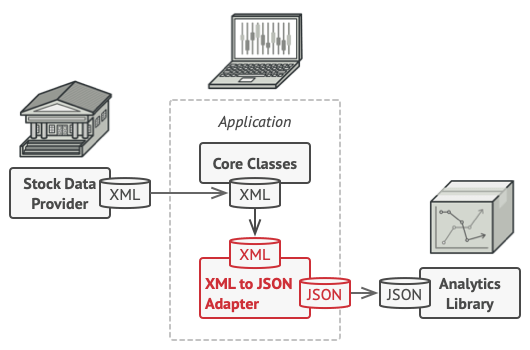
\includegraphics[scale=0.3]{./images/solution.png}
		\end{column}
	
		\begin{column}{.5\textwidth}
			\begin{itemize}
				\item You can create an adapter. This is a special object that converts the interface of one object so that another object can understand it.
				\item An adapter wraps one of the objects to hide the complexity of conversion happening behind the scenes. The wrapped object isn’t even aware of the adapter.
				\item Adapters can not only convert data into various formats but can also help objects with different interfaces collaborate. Here’s how it works:
				%The adapter gets an interface, compatible with one of the existing objects.
				%Using this interface, the existing object can safely call the adapter’s methods.
				%Upon receiving a call, the adapter passes the request to the second object, but in a format and order that the second object expects.
				\item Sometimes it’s even possible to create a two-way adapter that can convert the calls in both directions.
			\end{itemize}
		\end{column}
	\end{columns}
\end{frame}

\begin{frame}{The Intent of Adapter Design Pattern}
	\begin{center}
	\textcolor{red}{\textbf{Convert the interface of a class into another interface clients expect. Adapter lets classes work together that could not otherwise because of incompatible interfaces.}}\\
	\end{center}
\end{frame}

\begin{frame}{Structure of Adapter Pattern: Object adapter}
	\begin{center}
	\begin{tikzpicture}
 \umlemptyclass[x=0,y=0]{Client}
 \umlclass[x=4,y=0]{Client interface}{}{request()}
 \umlclass[x=4,y=-3]{Adapter}{}{request()}
 \umlclass[x=9,y=-3]{Adaptee}{}{specificRequest()}
 \umluniassoc[pos=0.95, align=right, name=uniassoc]{Client}{Client interface}
 \umluniassoc[pos=0.95, align=right, name=uniassoc]{Adapter}{Adaptee}
 \umlinherit{Adapter}{Client interface}
 \umlnote[x=4,y=-5, width=120]{Adapter}{Adaptee->specificRequest()}
	\end{tikzpicture}	
	\end{center}
\end{frame}

\begin{frame}{Basic implementation: Rectangle class}
\begin{columns}[T]
\begin{column}{.45\textwidth}
\lstset{basicstyle=\tiny,style=myCustomCppStyle}
rectangle.h
\lstinputlisting{./examples/squareRecAdapter/rectangle.h}
\end{column}

\begin{column}{.45\textwidth}
\lstset{basicstyle=\tiny,style=myCustomCppStyle}
rectangle.cpp
\lstinputlisting{./examples/squareRecAdapter/rectangle.cpp}
\end{column}
\end{columns}
\end{frame}

\begin{frame}{Basic implementation: Square class}
\begin{columns}[T]
\begin{column}{.45\textwidth}
\lstset{basicstyle=\tiny,style=myCustomCppStyle}
square.h
\lstinputlisting{./examples/squareRecAdapter/square.h}
\end{column}

\begin{column}{.45\textwidth}
\lstset{basicstyle=\tiny,style=myCustomCppStyle}
square.cpp
\lstinputlisting{./examples/squareRecAdapter/square.cpp}
\end{column}
\end{columns}
\end{frame}

\begin{frame}{Basic implementation: Adapter class}
\begin{columns}[T]
\begin{column}{.45\textwidth}
\lstset{basicstyle=\tiny,style=myCustomCppStyle}
adapter.h
\lstinputlisting{./examples/squareRecAdapter/adapter.h}
\end{column}

\begin{column}{.45\textwidth}
\lstset{basicstyle=\tiny,style=myCustomCppStyle}
adapter.cpp
\lstinputlisting{./examples/squareRecAdapter/adapter.cpp}
\end{column}
\end{columns}
\end{frame}

\begin{frame}{Basic implementation: client code}
\begin{columns}[T]
\begin{column}{.45\textwidth}
\lstset{basicstyle=\tiny,style=myCustomCppStyle}
main.cpp
\lstinputlisting{./examples/squareRecAdapter/main.cpp}
\end{column}

\begin{column}{.45\textwidth}
\lstset{basicstyle=\tiny,style=myCustomCppStyle}
\begin{itemize}
\item Object adapter
\end{itemize}
\end{column}
\end{columns}
\end{frame}

\begin{frame}{Structure of Adapter Pattern: Class adapter}
	\begin{center}
	\begin{tikzpicture}
 \umlemptyclass[x=0,y=0]{Client}
 \umlclass[x=4,y=0]{Client interface}{}{request()}
 \umlclass[x=9,y=0]{Adaptee}{}{specificRequest()}
 \umlclass[x=6.5,y=-4]{Adapter}{}{request()}
 \umluniassoc[pos=0.95, align=right, name=uniassoc]{Client}{Client interface}
 \umlinherit[geometry=|-|]{Adapter}{Client interface}
 \umlinherit[geometry=|-|]{Adapter}{Adaptee}
 \umlnote[x=3,y=-5, width=100]{Adapter}{specificRequest()}
	\end{tikzpicture}	
	\end{center}
\end{frame}

\begin{frame}{Basic implementation: Rectangle class}
\begin{columns}[T]
\begin{column}{.45\textwidth}
\lstset{basicstyle=\tiny,style=myCustomCppStyle}
rectangle.h
\lstinputlisting{./examples/classAdapter/rectangle.h}
\end{column}

\begin{column}{.45\textwidth}
\lstset{basicstyle=\tiny,style=myCustomCppStyle}
rectangle.cpp
\lstinputlisting{./examples/classAdapter/rectangle.cpp}
\end{column}
\end{columns}
\end{frame}

\begin{frame}{Basic implementation: Square class}
\begin{columns}[T]
\begin{column}{.45\textwidth}
\lstset{basicstyle=\tiny,style=myCustomCppStyle}
square.h
\lstinputlisting{./examples/classAdapter/square.h}
\end{column}

\begin{column}{.45\textwidth}
\lstset{basicstyle=\tiny,style=myCustomCppStyle}
square.cpp
\lstinputlisting{./examples/classAdapter/square.cpp}
\end{column}
\end{columns}
\end{frame}

\begin{frame}{Basic implementation: Adapter class}
\begin{columns}[T]
\begin{column}{.45\textwidth}
\lstset{basicstyle=\tiny,style=myCustomCppStyle}
adapter.h
\lstinputlisting{./examples/classAdapter/adapter.h}
\end{column}

\begin{column}{.45\textwidth}
\lstset{basicstyle=\tiny,style=myCustomCppStyle}
adapter.cpp
\lstinputlisting{./examples/classAdapter/adapter.cpp}
\end{column}
\end{columns}
\end{frame}

\begin{frame}{Basic implementation: client code}
\begin{columns}[T]
\begin{column}{.45\textwidth}
	\lstset{basicstyle=\tiny,style=myCustomCppStyle}
	main.cpp
	\lstinputlisting{./examples/classAdapter/main.cpp}
\end{column}

\begin{column}{.5\textwidth}
	\lstset{basicstyle=\tiny,style=myCustomCppStyle}
	\begin{itemize}
		\item This implementation uses inheritance: the adapter inherits interfaces from both objects at the same time.
		\item The Class Adapter doesn’t need to wrap any objects because it inherits behaviors from both the client and the service. The adaptation happens within the overridden methods. The resulting adapter can be used in place of an existing client class.
	\end{itemize}
\end{column}
\end{columns}
\end{frame}

\begin{frame}{Applicability}
	\begin{itemize}
		\setlength\itemsep{1em}
		\item Use the Adapter class when you want to use some existing class, but its interface isn’t compatible with the rest of your code.
		\item The Adapter pattern lets you create a middle-layer class that serves as a translator between your code and a legacy class, a 3rd-party class or any other class with a weird interface.
		\item Use the pattern when you want to reuse several existing subclasses that lack some common functionality that can’t be added to the superclass.
		\item You could extend each subclass and put the missing functionality into new child classes. However, you’ll need to duplicate the code across all of these new classes, which smells really bad.
		% The much more elegant solution would be to put the missing functionality into an adapter class. Then you would wrap objects with missing features inside the adapter, gaining needed features dynamically. For this to work, the target classes must have a common interface, and the adapter’s field should follow that interface. This approach looks very similar to the Decorator pattern.
	\end{itemize}
\end{frame}

\begin{frame}{How to Implement}
	\begin{itemize}
		\setlength\itemsep{1em}
		\item Make sure that you have at least two classes with incompatible interfaces:
		\begin{itemize}
		\item A useful service class, which you can’t change (often 3rd-party, legacy or with lots of existing dependencies).
		\item One or several client classes that would benefit from using the service class.
		\end{itemize}
		\item Declare the client interface and describe how clients communicate with the service.
		\item Create the adapter class and make it follow the client interface. Leave all the methods empty for now.
	\end{itemize}
\end{frame}

\begin{frame}{How to Implement}
	\begin{itemize}
		\setlength\itemsep{1em}
		\item Add a field to the adapter class to store a reference to the service object. The common practice is to initialize this field via the constructor, but sometimes it’s more convenient to pass it to the adapter when calling its methods.
		\item One by one, implement all methods of the client interface in the adapter class. The adapter should delegate most of the real work to the service object, handling only the interface or data format conversion.
		\item Clients should use the adapter via the client interface. This will let you change or extend the adapters without affecting the client code.
	\end{itemize}
\end{frame}

\begin{frame}{Pros and Cons}
	\begin{columns}[T]
		\begin{column}{.5\textwidth}
			\begin{itemize}
				\item  Single Responsibility Principle. You can separate the interface or data conversion code from the primary business logic of the program.
				\item pen/Closed Principle. You can introduce new types of adapters into the program without breaking the existing client code, as long as they work with the adapters through the client interface.
			\end{itemize}
		\end{column}
	
		\begin{column}{.5\textwidth}
			\begin{itemize}
				\item The overall complexity of the code increases because you need to introduce a set of new interfaces and classes. Sometimes it’s simpler just to change the service class so that it matches the rest of your code.
			\end{itemize}
		\end{column}
	\end{columns}
\end{frame}

\begin{frame}{Relations with Other Patterns}
	\begin{itemize}
		\setlength\itemsep{1em}
		\item Bridge is usually designed up-front, letting you develop parts of an application independently of each other. On the other hand, Adapter is commonly used with an existing app to make some otherwise-incompatible classes work together nicely.
		\item Adapter changes the interface of an existing object, while Decorator enhances an object without changing its interface. In addition, Decorator supports recursive composition, which isn’t possible when you use Adapter.
		\item Adapter provides a different interface to the wrapped object, Proxy provides it with the same interface, and Decorator provides it with an enhanced interface.
	\end{itemize}
\end{frame}

\begin{frame}{Relations with Other Patterns}
	\begin{itemize}
		\setlength\itemsep{1em}
		\item Facade defines a new interface for existing objects, whereas Adapter tries to make the existing interface usable. Adapter usually wraps just one object, while Facade works with an entire subsystem of objects.
		\item Bridge, State, Strategy (and to some degree Adapter) have very similar structures. Indeed, all of these patterns are based on composition, which is delegating work to other objects. However, they all solve different problems. A pattern isn’t just a recipe for structuring your code in a specific way. It can also communicate to other developers the problem the pattern solves.
	\end{itemize}
\end{frame}

\begin{frame}
\begin{center}
{\fontsize{40}{50}\selectfont Thank You!}
\end{center}
\end{frame}

\end{document}
